\chapter{Depth estimation}


\begin{description}
    \item[Stereo correspondence] \marginnote{Stereo correspondence}
        Given an ideal stereo setup, the depth of each point in the world can be obtained by solving a correspondence problem along rows. Given two points $(u_L, v_L)$ and $(u_R, v_R=v_L)$ in the left and right image, respectively, representing the projection of the same 3D point, its distance $z$ from the camera can be determined using the disparity $d$:
        \[
            \begin{gathered}
                d = u_L - u_R \\
                z = \frac{bf}{d}
            \end{gathered}
        \]
        where $b$ is the baseline (i.e., camera distance) and $f$ is the focal length.

        \begin{figure}[H]
            \centering
            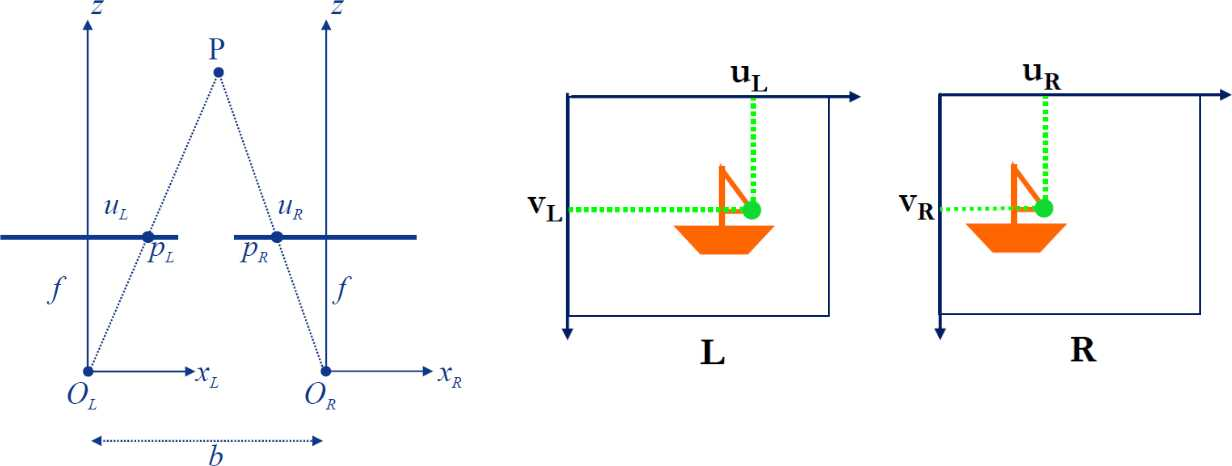
\includegraphics[width=0.65\linewidth]{./img/stereo_correspondence.jpg}
        \end{figure}
\end{description}

\begin{remark}
    Due to the lack of data, existing models are trained on synthetic data and fine-tuned afterwards on real data.
\end{remark}



\section{Monocular depth estimation}

\begin{description}
    \item[Monocular (single-view) depth estimation] \marginnote{Monocular (single-view) depth estimation}
        Reconstruct the 3D structure of a scene from a single image.

        \begin{remark}
            In principle, this is an ill-posed problem. However, humans are able to solve it through learning.
        \end{remark}
\end{description}


\begin{remark}
    Traditional supervised frameworks (e.g., encoder-decoder) to solve monocular depth estimation have some limitations:
    \begin{itemize}
        \item They require a large amount of realistic synthetic data.
        \item They require expensive hardware for depth measurement when fine-tuning on real data.
    \end{itemize}
\end{remark}


\subsection{Monodepth}

\begin{description}
    \item[Supervised stereo pipeline] \marginnote{Supervised stereo pipeline}
        \phantom{}
        \begin{description}
            \item[Naive approach] 
                A possible solution for depth estimation is to feed a CNN with a pair of synchronized images and make it predict the left (or right) disparity. However, this approach requires to know the ground-truth disparity, which is expensive to obtain.

                \begin{figure}[H]
                    \centering
                    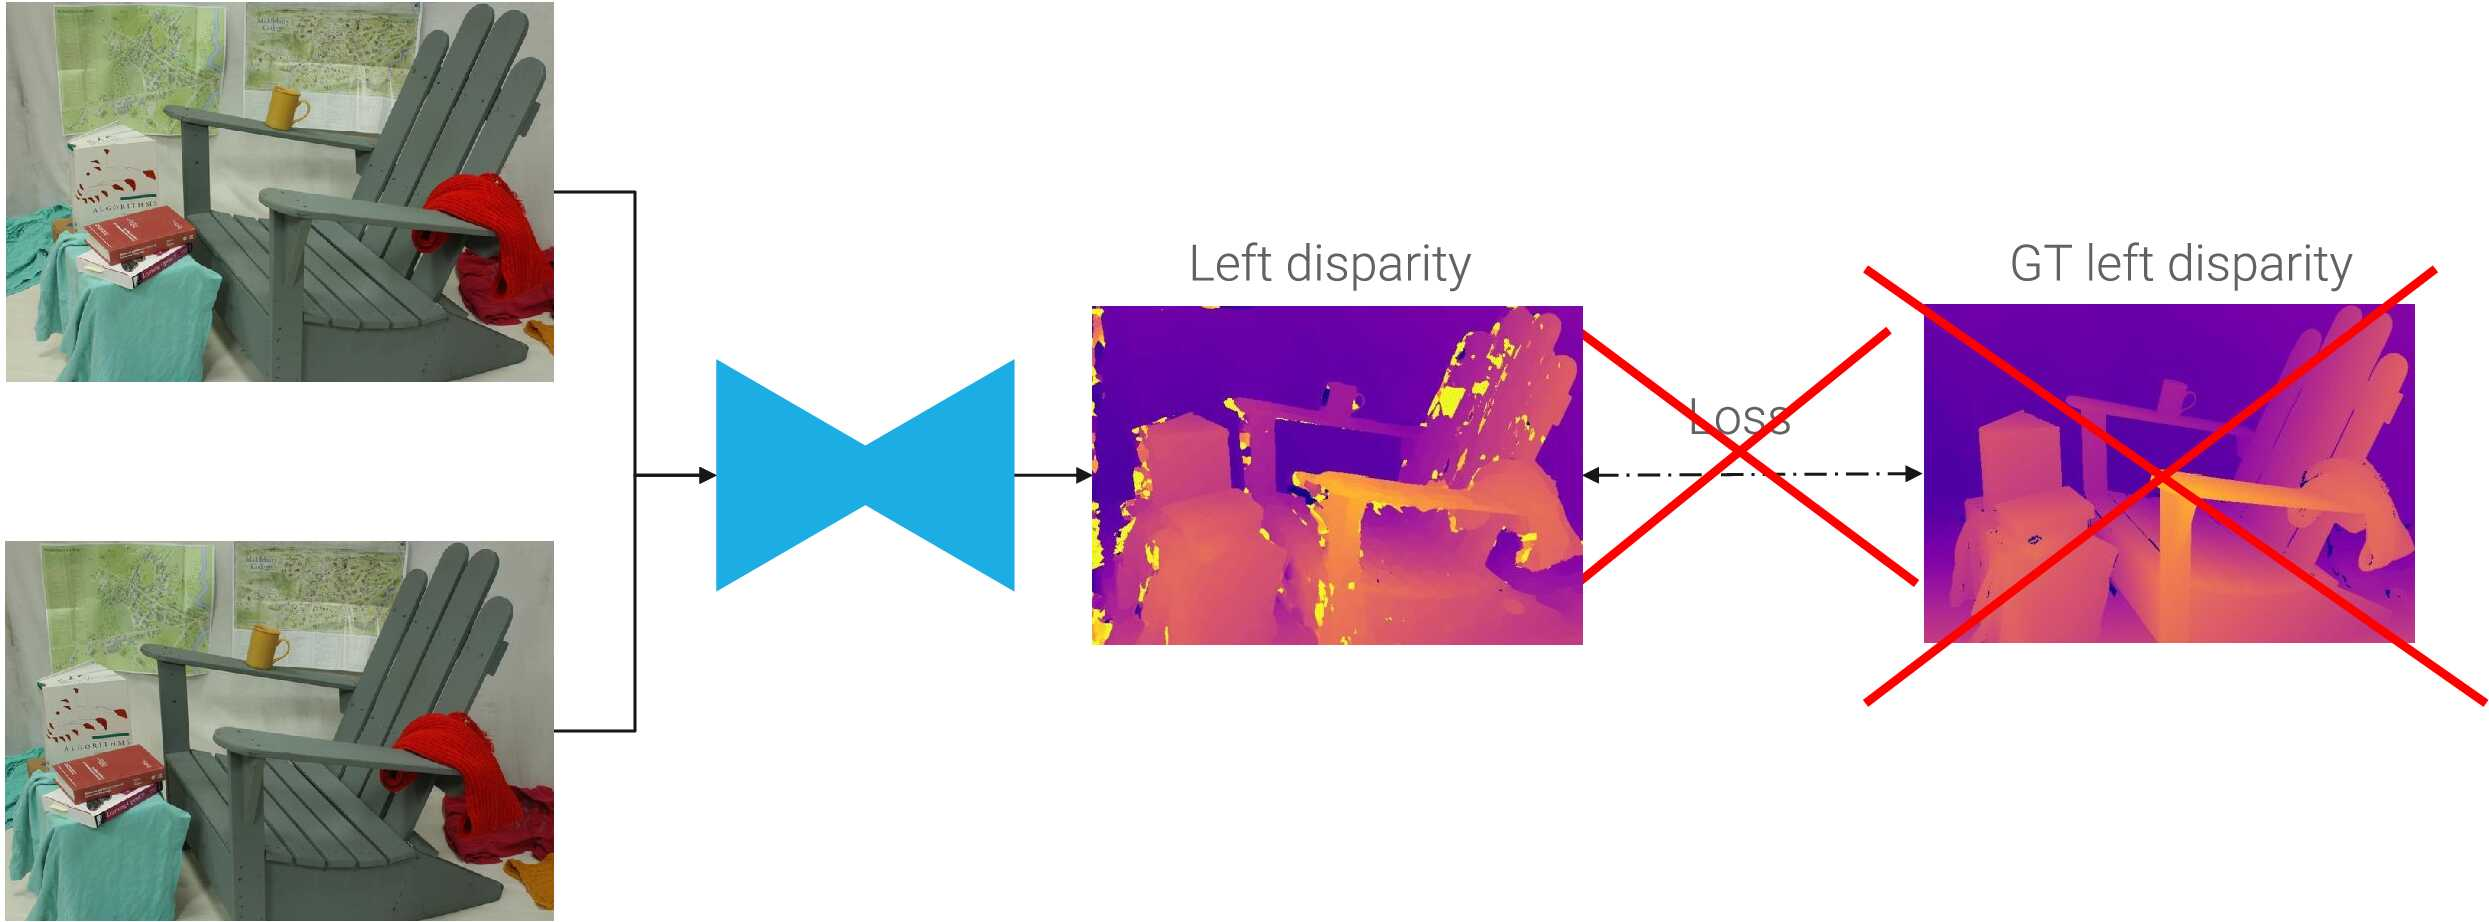
\includegraphics[width=0.7\linewidth]{./img/_stereo_pipeline_naive.jpg}
                \end{figure}

            \item[Reconstruction approach]
                Make the model predict the left disparity which is then used to reconstruct the right image. This works as a pixel $(u, v)$ in the left image with disparity $\tilde{d}$ should appear as the same to the pixel $(u+\tilde{d}, v)$ in the right image.

                \begin{figure}[H]
                    \centering
                    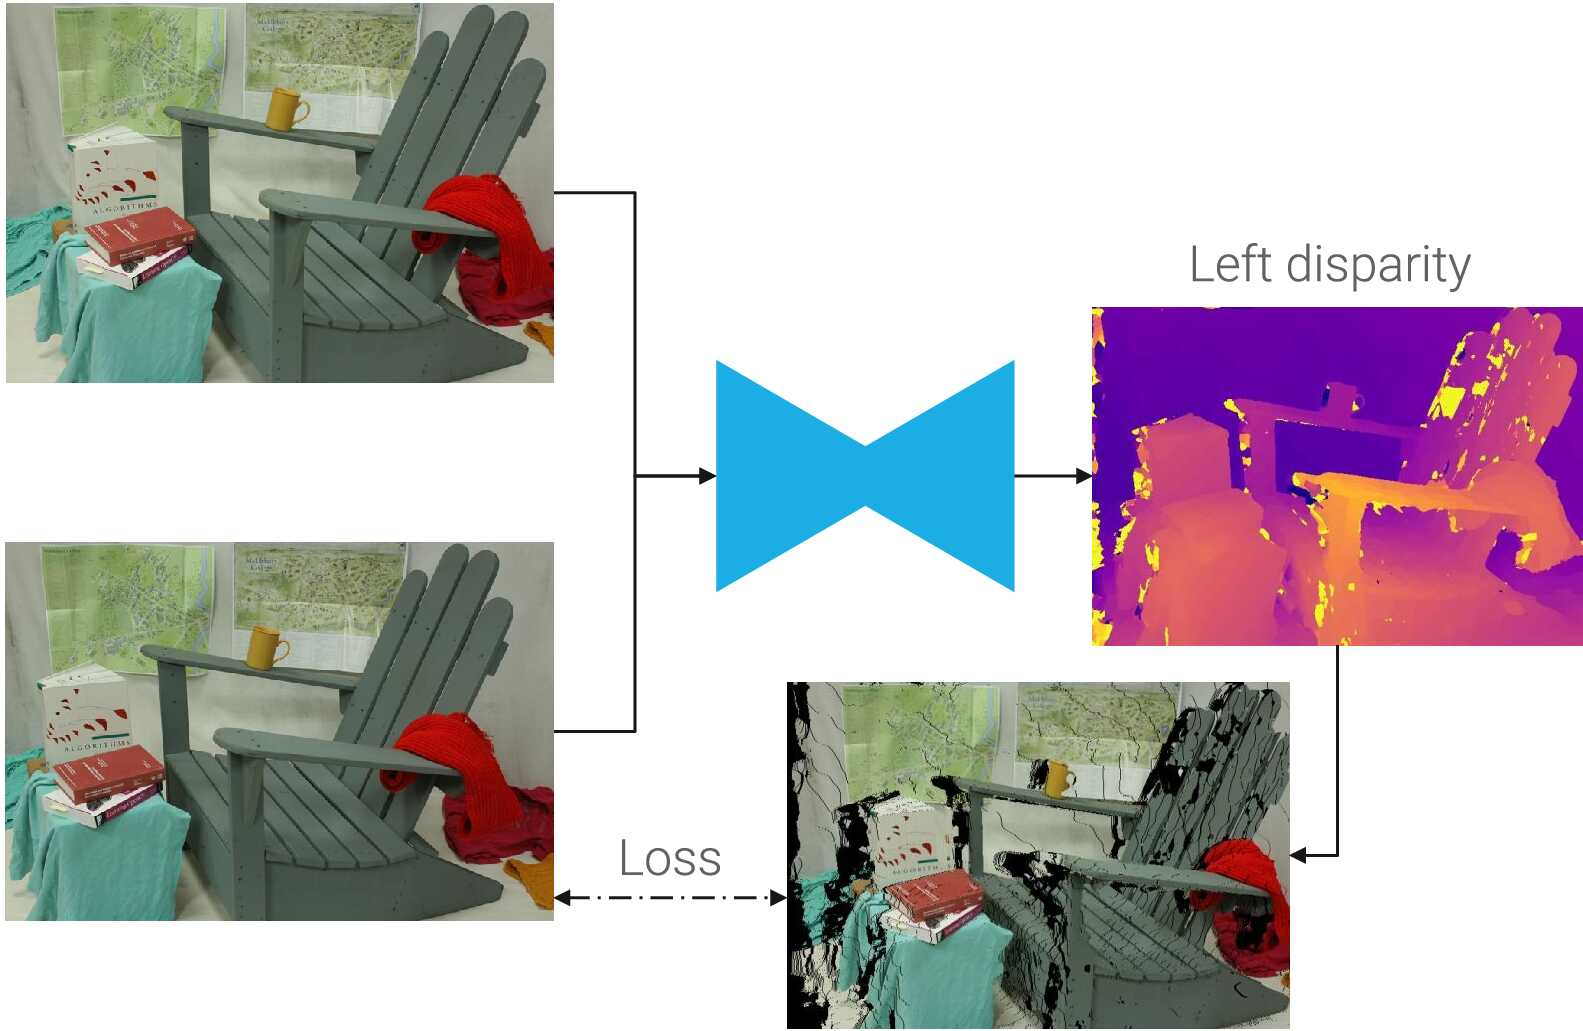
\includegraphics[width=0.45\linewidth]{./img/_stereo_pipeline_reconstruction.jpg}
                \end{figure}
        \end{description}
\end{description}

\begin{description}
    \item[Monodepth (no left-right)] \marginnote{Monodepth (no left-right)}
        Network that takes as input the left (or right) image of a stereo vision system and predicts the left (or right) disparity.

        \begin{description}
            \item[Training (naive)] 
                Once the left disparity has been predicted, it is used to reconstruct the right image.

                \begin{figure}[H]
                    \centering
                    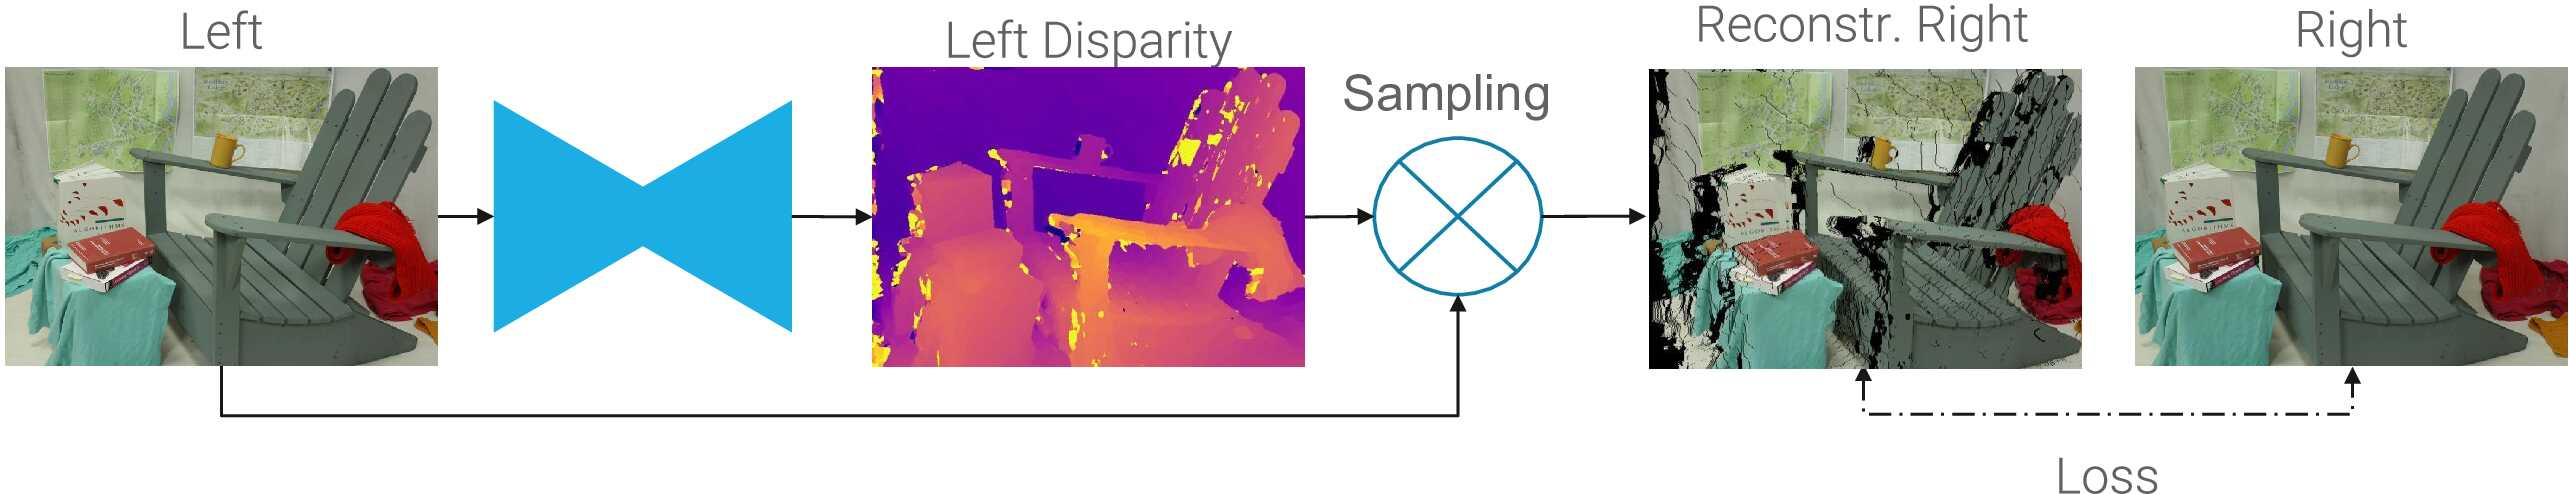
\includegraphics[width=0.8\linewidth]{./img/_monodepth_naive.jpg}
                    \caption{Naive training flow}
                \end{figure}

                \begin{remark}
                    Forward mapping creates holes and is ambiguous as disparities are non-integer values.
                \end{remark}

                \begin{description}
                    \item[(Backward) bilinear sampling] 
                        Compute the right image by determining each pixel of the output backwards and by interpolating it in the left image.

                        \begin{remark}
                            By reconstructing the right image backwards, the estimated disparity will be with respect to the right image, which is not available during inference.
                        \end{remark}

                        \begin{figure}[H]
                            \centering
                            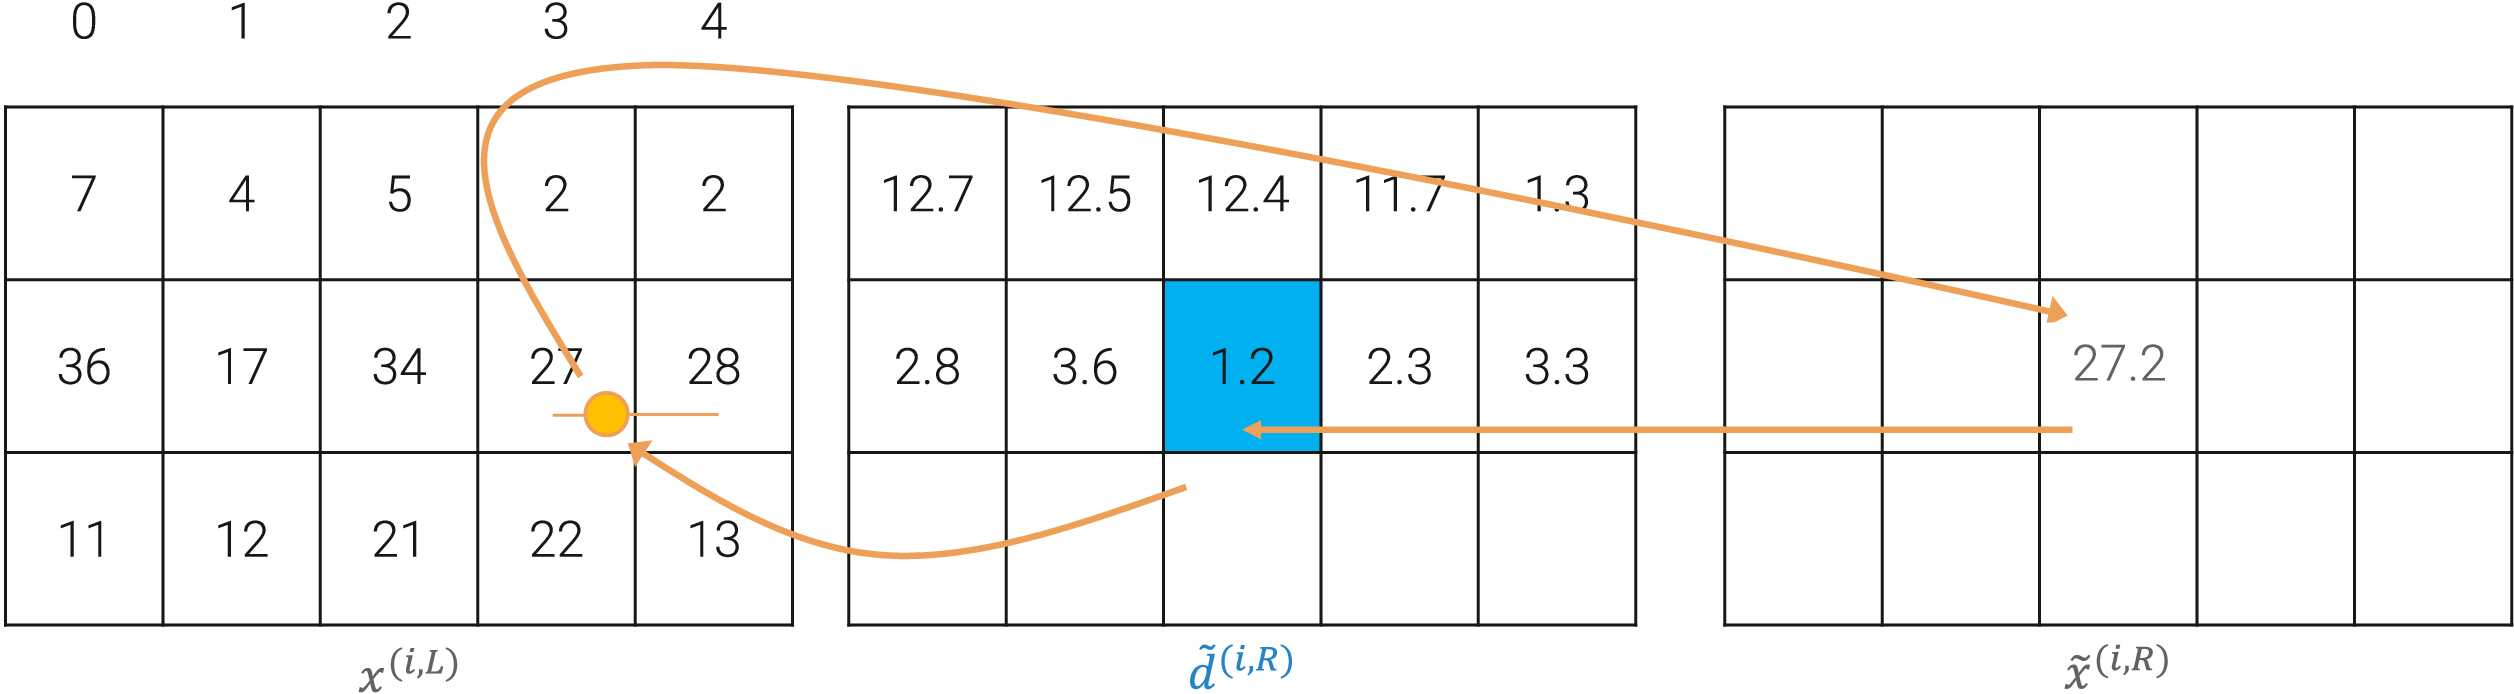
\includegraphics[width=0.65\linewidth]{./img/_monodepth_train_naive.jpg}
                            \caption{Backward reconstruction from the right image}
                        \end{figure}
                \end{description}

            \item[Training (correct)] 
                Once the left disparity has been predicted, it is used to reconstruct the left image by backward mapping from the right image (which is available at train time).

                \begin{figure}[H]
                    \centering
                    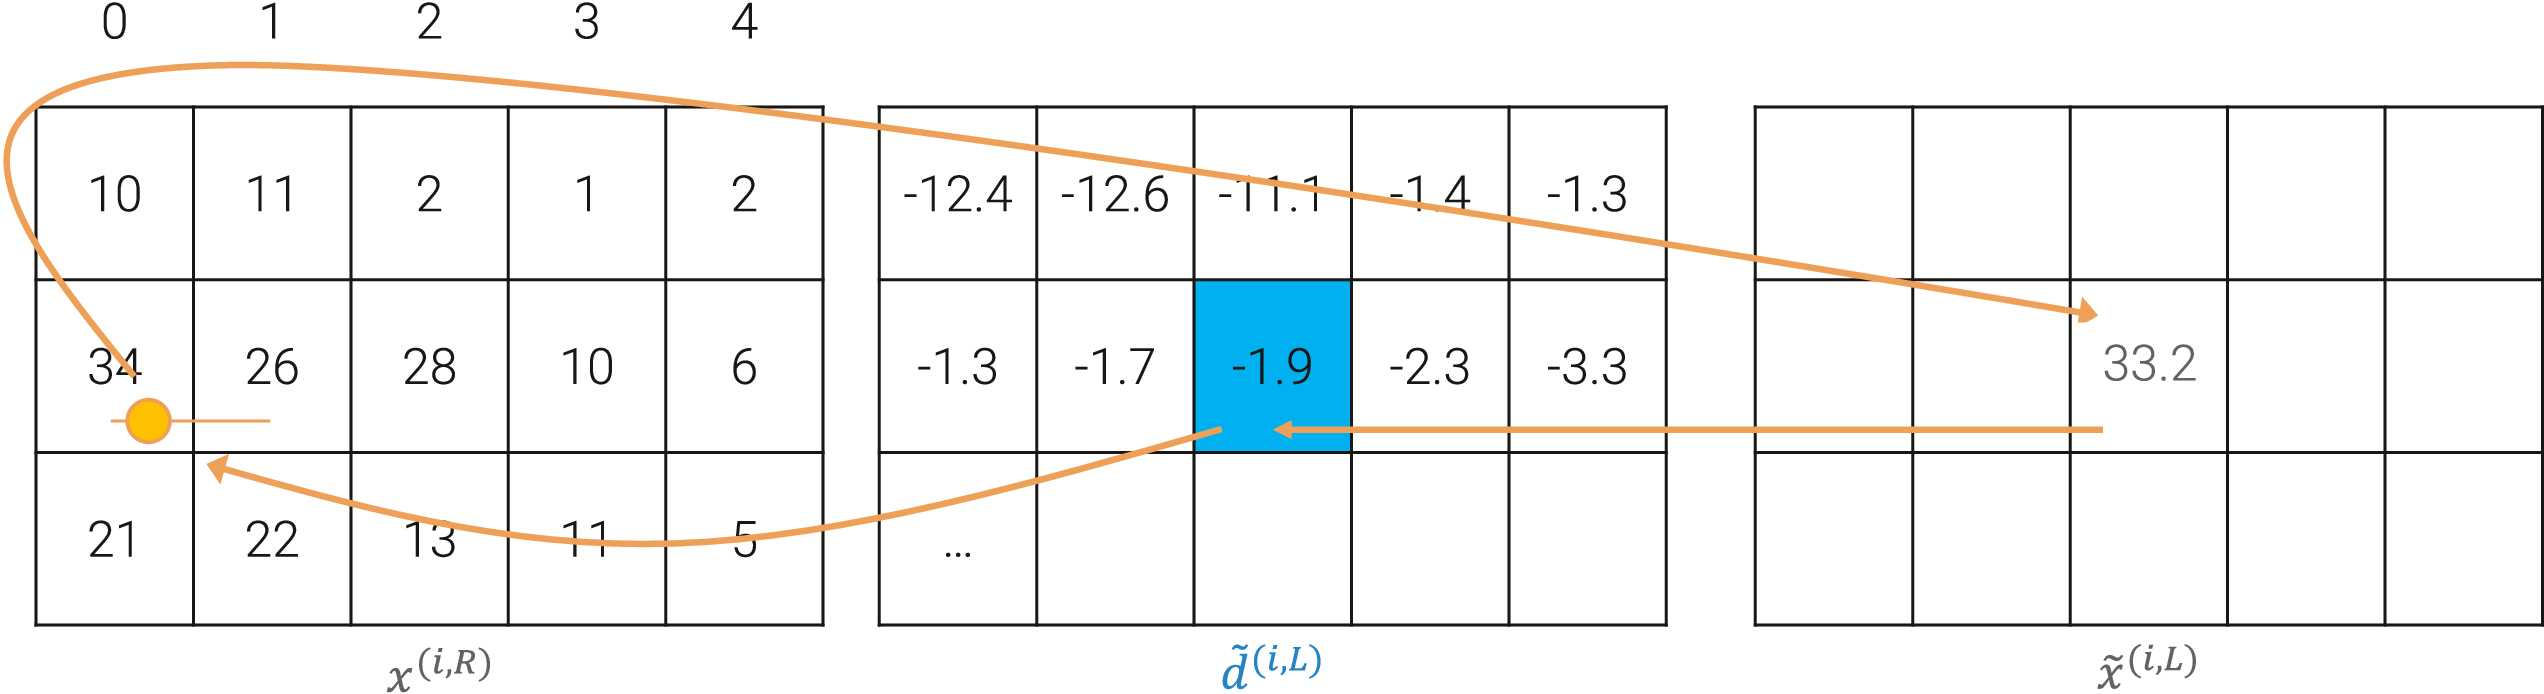
\includegraphics[width=0.65\linewidth]{./img/_monodepth_train_correct.jpg}
                    \caption{Backward reconstruction from the left image}
                \end{figure}

                \begin{figure}[H]
                    \centering
                    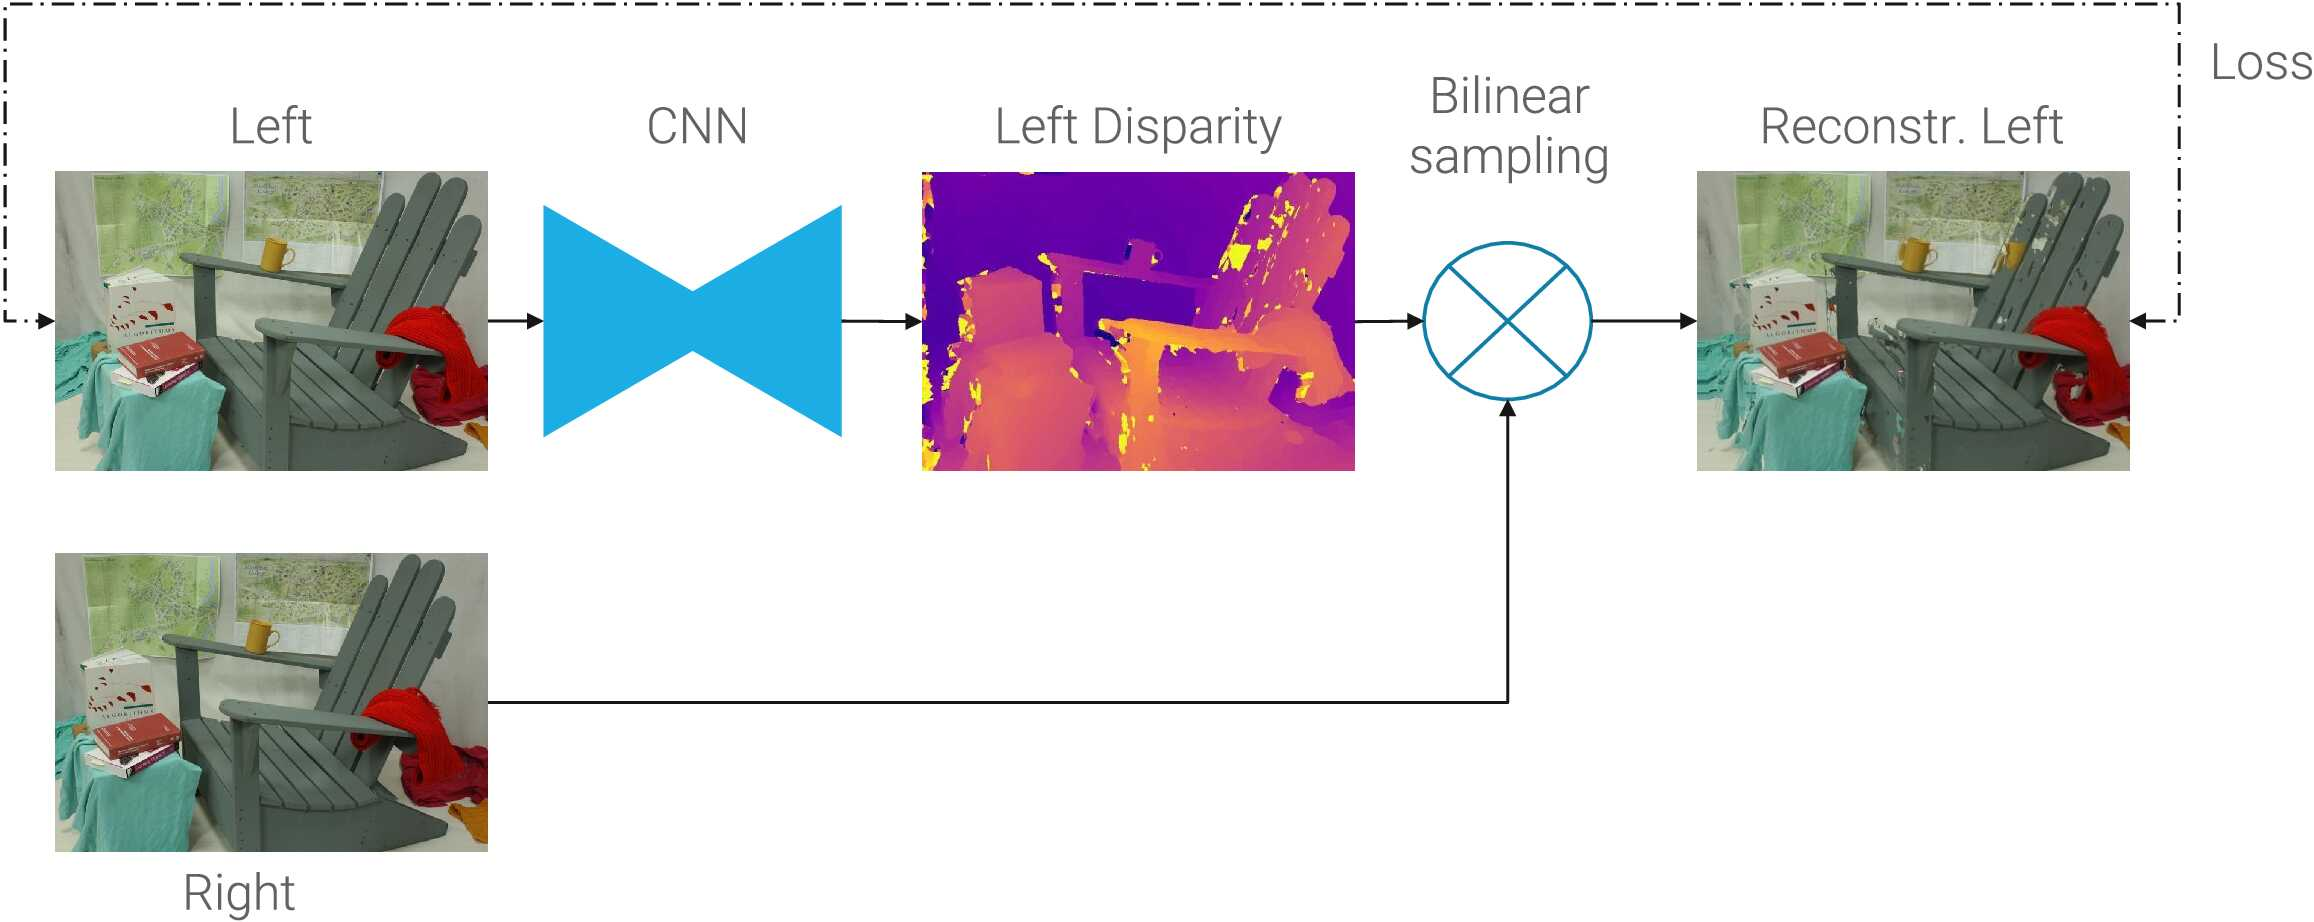
\includegraphics[width=0.7\linewidth]{./img/_monodepth_correct.jpg}
                    \caption{Actual training flow}
                \end{figure}

                \begin{description}
                    \item[Reconstruction loss] \marginnote{Reconstruction loss}
                        Mix between the structural similarity index (SSIM) (which measures a perceptual distance) and L1 norm:
                        \[ \mathcal{L}_{\text{ap}}(x^{(i, L)}) = \frac{1}{N} \sum_{(u, v)} \left( \alpha \frac{1-\texttt{SSIM}(x_{u, v}^{(i, L)}, \hat{x}_{u, v}^{(i, L)})}{2} + (1-\alpha) \left\Vert x_{u, v}^{(i, L)} - \hat{x}_{u, v}^{(i, L)} \right\Vert_1 \right) \]
                        where $x^{(i, L)}$ is the $i$-th input left image and $\hat{x}^{(i, L)}$ the reconstructed left image.

                    \item[Disparity smoothness] \marginnote{Disparity smoothness}
                        Loss penalty to exploit the fact that disparity tends to be locally smooth and only change at edges:
                        \[ \mathcal{L}_{\text{ds}}(x^{(i, L)}) = \frac{1}{N} \sum_{(u, v)} \left(\left\vert \partial_u d_{u, v}^{(i, L)} \right\vert e^{- \Vert \partial_u x_{u, v}^{(i, L)} \Vert_1} + \left\vert \partial_v d_{u, v}^{(i, L)} \right\vert e^{- \Vert \partial_v x_{u, v}^{(i, L)} \Vert_1} \right) \]
                        where $x^{(i, L)}$ is the $i$-th input left image and $d^{(i, L)}$ the predicted left disparity.

                        In this way:
                        \begin{itemize}
                            \item If the gradient of $x_{u, v}^{(i, L)}$ is small (i.e., $e^{- \Vert \partial_* x_{u, v}^{(i, L)} \Vert_1} \rightarrow 1$), the gradient of $d_{u, v}^{(i, L)}$ is forced to be small too.
                            \item If the gradient of $x_{u, v}^{(i, L)}$ is big (i.e., $e^{- \Vert \partial_* x_{u, v}^{(i, L)} \Vert_1} \rightarrow 0$), the gradient of $d_{u, v}^{(i, L)}$ can be indifferently large or small.
                        \end{itemize}
                \end{description}
        \end{description}

        \begin{remark}
            Monodepth without left-right processing has fairly good results but it exhibits texture-copy artifacts and errors at depth discontinuities.

            \begin{figure}[H]
                \centering
                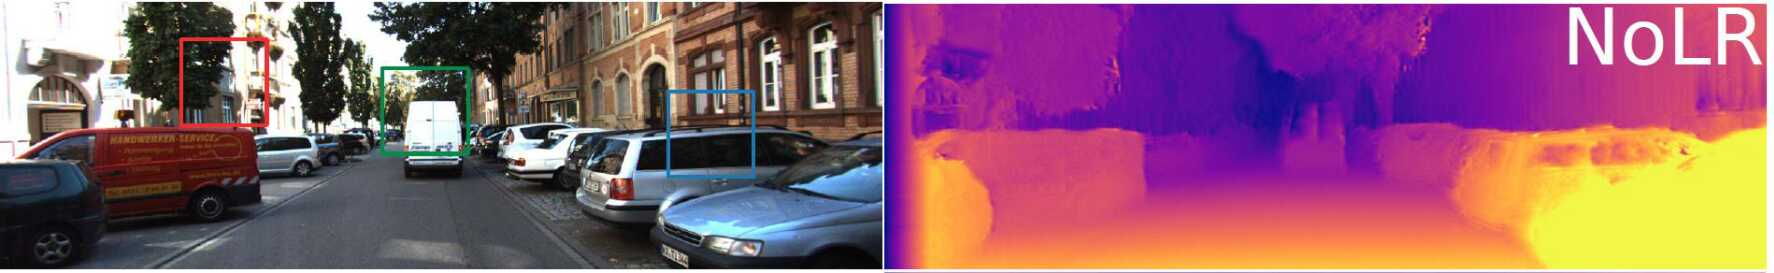
\includegraphics[width=0.9\linewidth]{./img/monodepth_no_lr_results.jpg}
            \end{figure}
        \end{remark}

        \begin{remark}
            Monodepth in this form requires stereo images but only exploits one of the images.
        \end{remark}


    \item[Monodepth (left-right)] \marginnote{Monodepth (left-right)}
        Make the network predict both left and right disparity and reconstruct both left and right images.

        \begin{description}
            \item[Disparity consistency loss] \marginnote{Disparity consistency loss}
                Enforces that the shifts of the two estimated disparities are consistent:
                \[ \mathcal{L}_{\text{lr}}(x^{(i, L)}, x^{(i, R)}) = \frac{1}{N} \sum_{(u, v)} \left| d_{u, v}^{(i, L)} - d^{(i, R)}_{u+d_{u, v}^{(i, L)}, v} \right| + \frac{1}{N} \sum_{(u, v)} \left| d_{u+d_{u, v}^{(i, R)}, v}^{(i, L)} - d^{(i, R)}_{u, v} \right| \]
                where $d^{(i, L)}$ and $d^{(i, R)}$ are the $i$-th left and right predicted disparity, respectively.

                The overall loss is the following:
                \[ 
                    \begin{split}
                        \mathcal{L}(x^{(i, L)}, x^{(i, R)}) = &\,\alpha_\text{ap} \left( \mathcal{L}_\text{ap}(x^{(i, L)}) + \mathcal{L}_\text{ap}(x^{(i, R)}) \right) \\
                            &+ \alpha_\text{ds} \left( \mathcal{L}_\text{ds}(x^{(i, L)}) + \mathcal{L}_\text{ds}(x^{(i, R)}) \right) \\
                            &+ \alpha_\text{lr} \mathcal{L}_\text{lr}(x^{(i, L)}, x^{(i, R)})
                    \end{split}
                \]

                \begin{figure}[H]
                    \centering
                    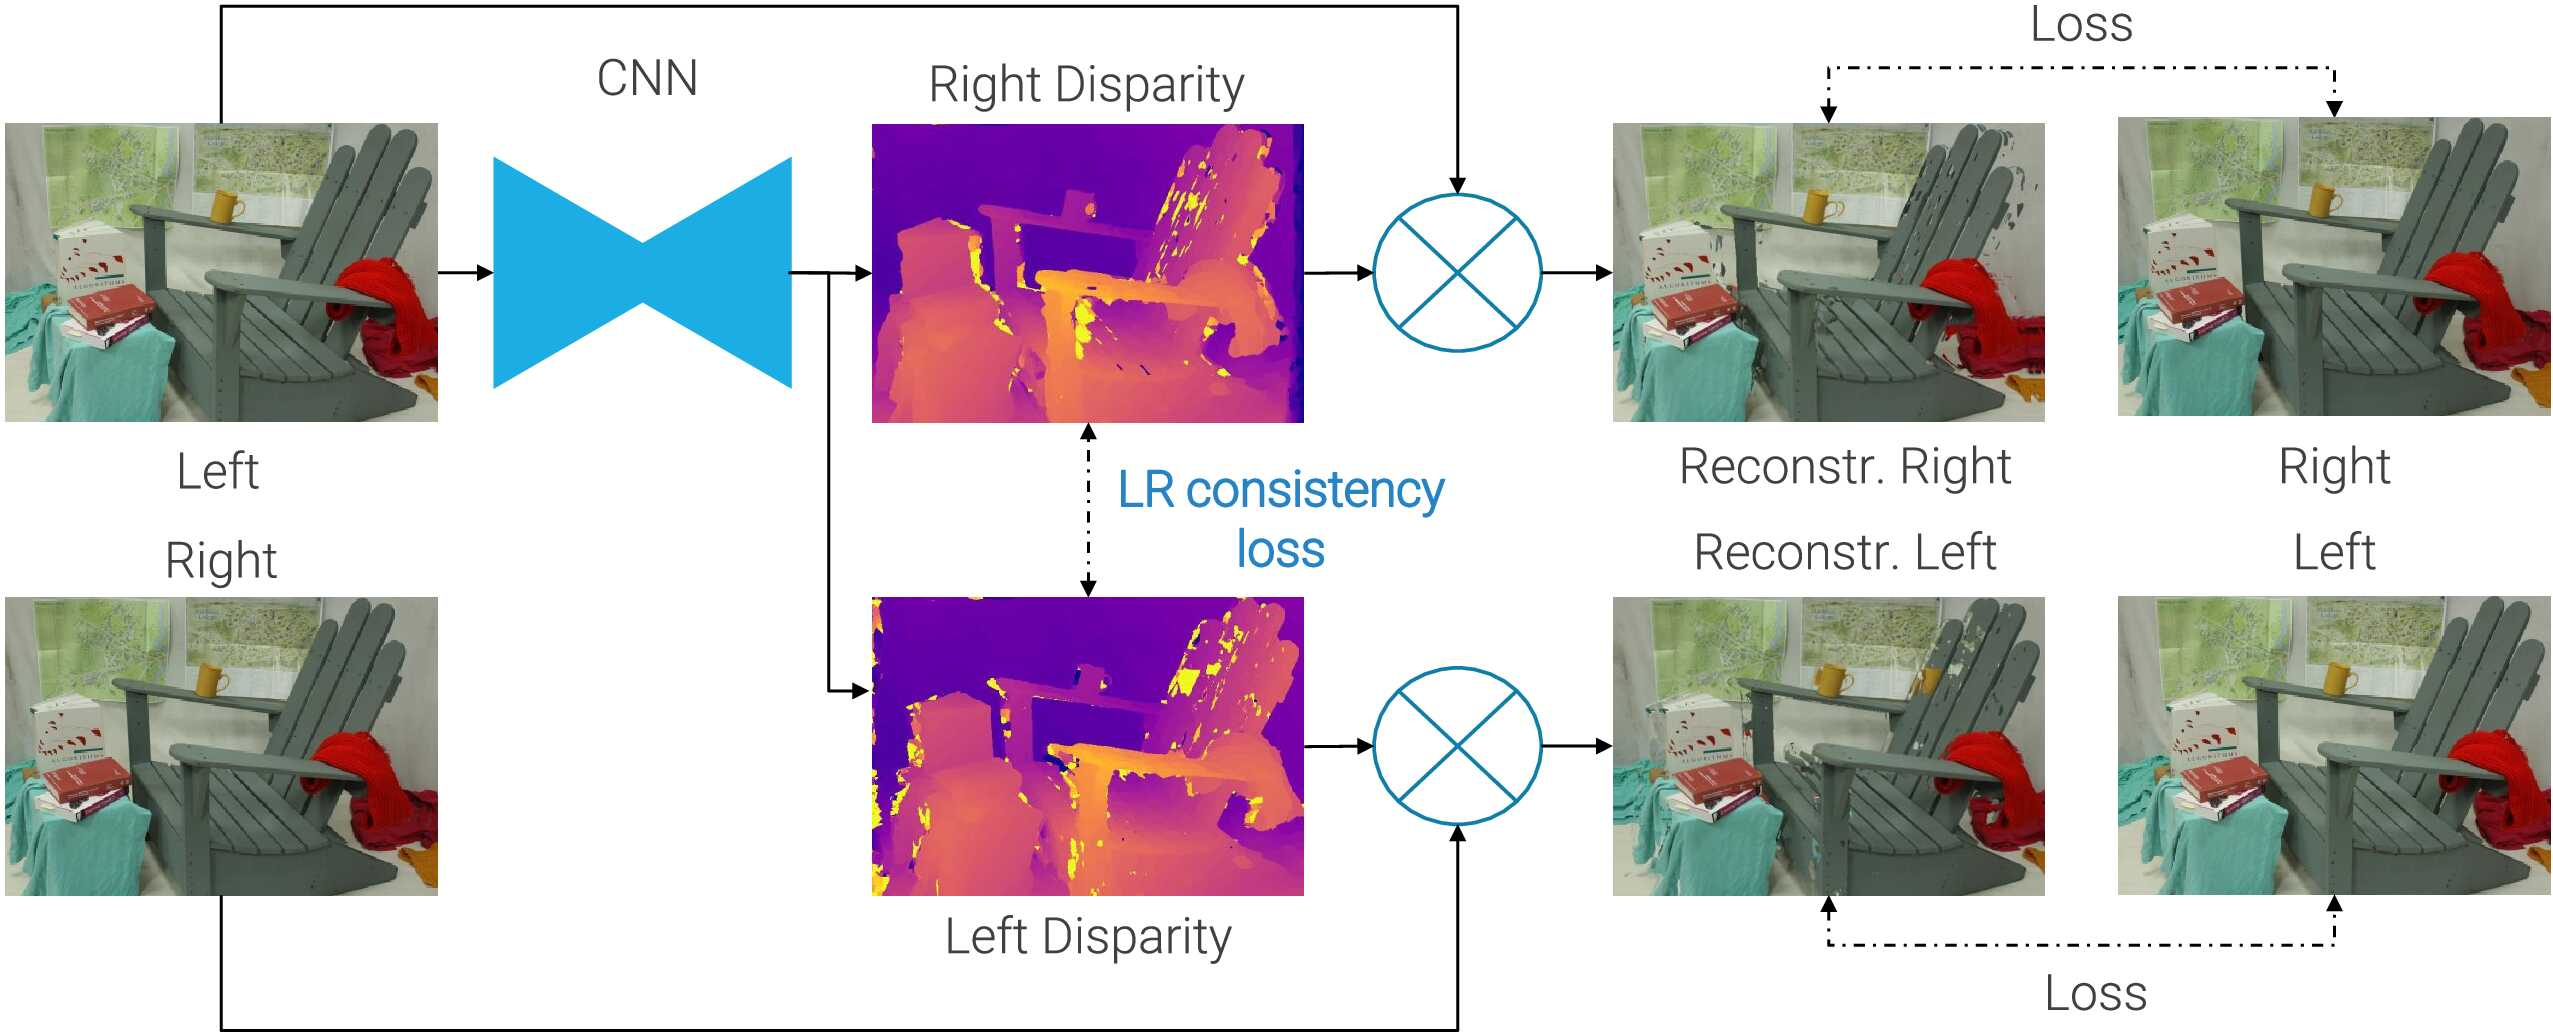
\includegraphics[width=0.7\linewidth]{./img/_monodepth_lr.jpg}
                \end{figure}

            \item[Inference]
                Use the left disparity to determine depth. Everything else is not necessary.

            \item[Architecture]
                Monodepth is implemented as a U-Net like network:
                \begin{itemize}
                    \item Up-convolutions are substituted with bilinear up-sampling to avoid checkerboard artifacts.
                    \item Disparity maps are computed at several resolutions and processed by the loss for alignment reason.
                \end{itemize}

                \begin{remark}
                    It has been seen that better encoders help performance.
                \end{remark}

            \begin{figure}[H]
                \centering
                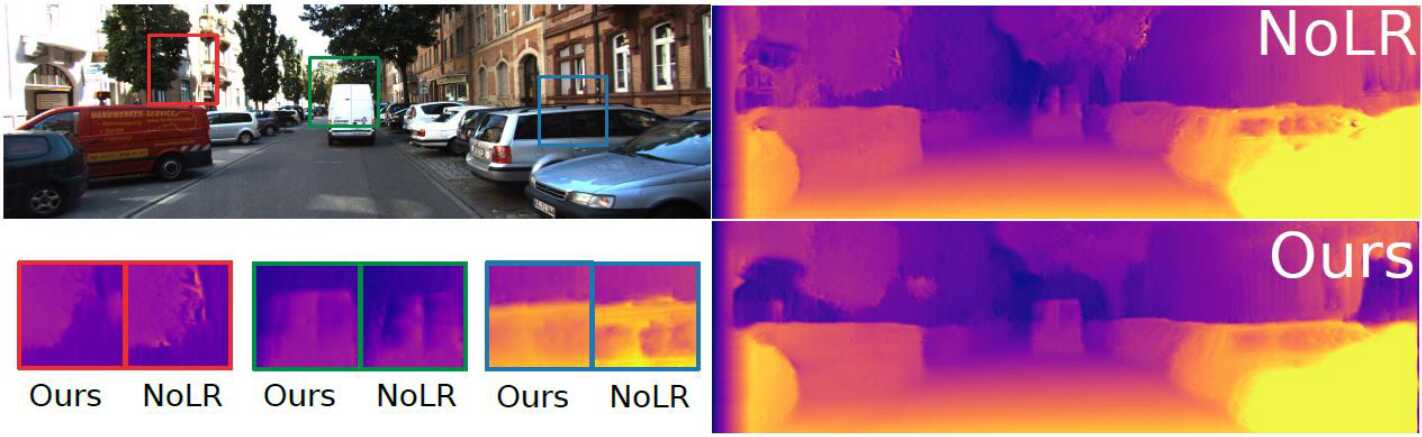
\includegraphics[width=0.7\linewidth]{./img/monodepth_lr_results.jpg}
                \caption{Comparison of Monodepth with and without left-right processing}
            \end{figure}
        \end{description}
    \end{description}


\subsection{Structure from motion learner}

\begin{description}
    \item[Structure from motion learner (SfMLearner)] \marginnote{Structure from motion learner (SfMLearner)}
        Relaxes the assumption of stereo images by using monocular video frames.

        The network takes as input a target image and nearby image(s) and is based on two flows:
        \begin{descriptionlist}
            \item[Depth CNN] Takes as input the target image and estimates its depth map.

            \item[Pose CNN] Takes as input the target and nearby images, and estimates the camera poses to project from target to nearby image.
        \end{descriptionlist}
        The outputs of both networks are used to reconstruct the target image and a reconstruction loss is used for training.

        \begin{figure}[H]
            \centering
            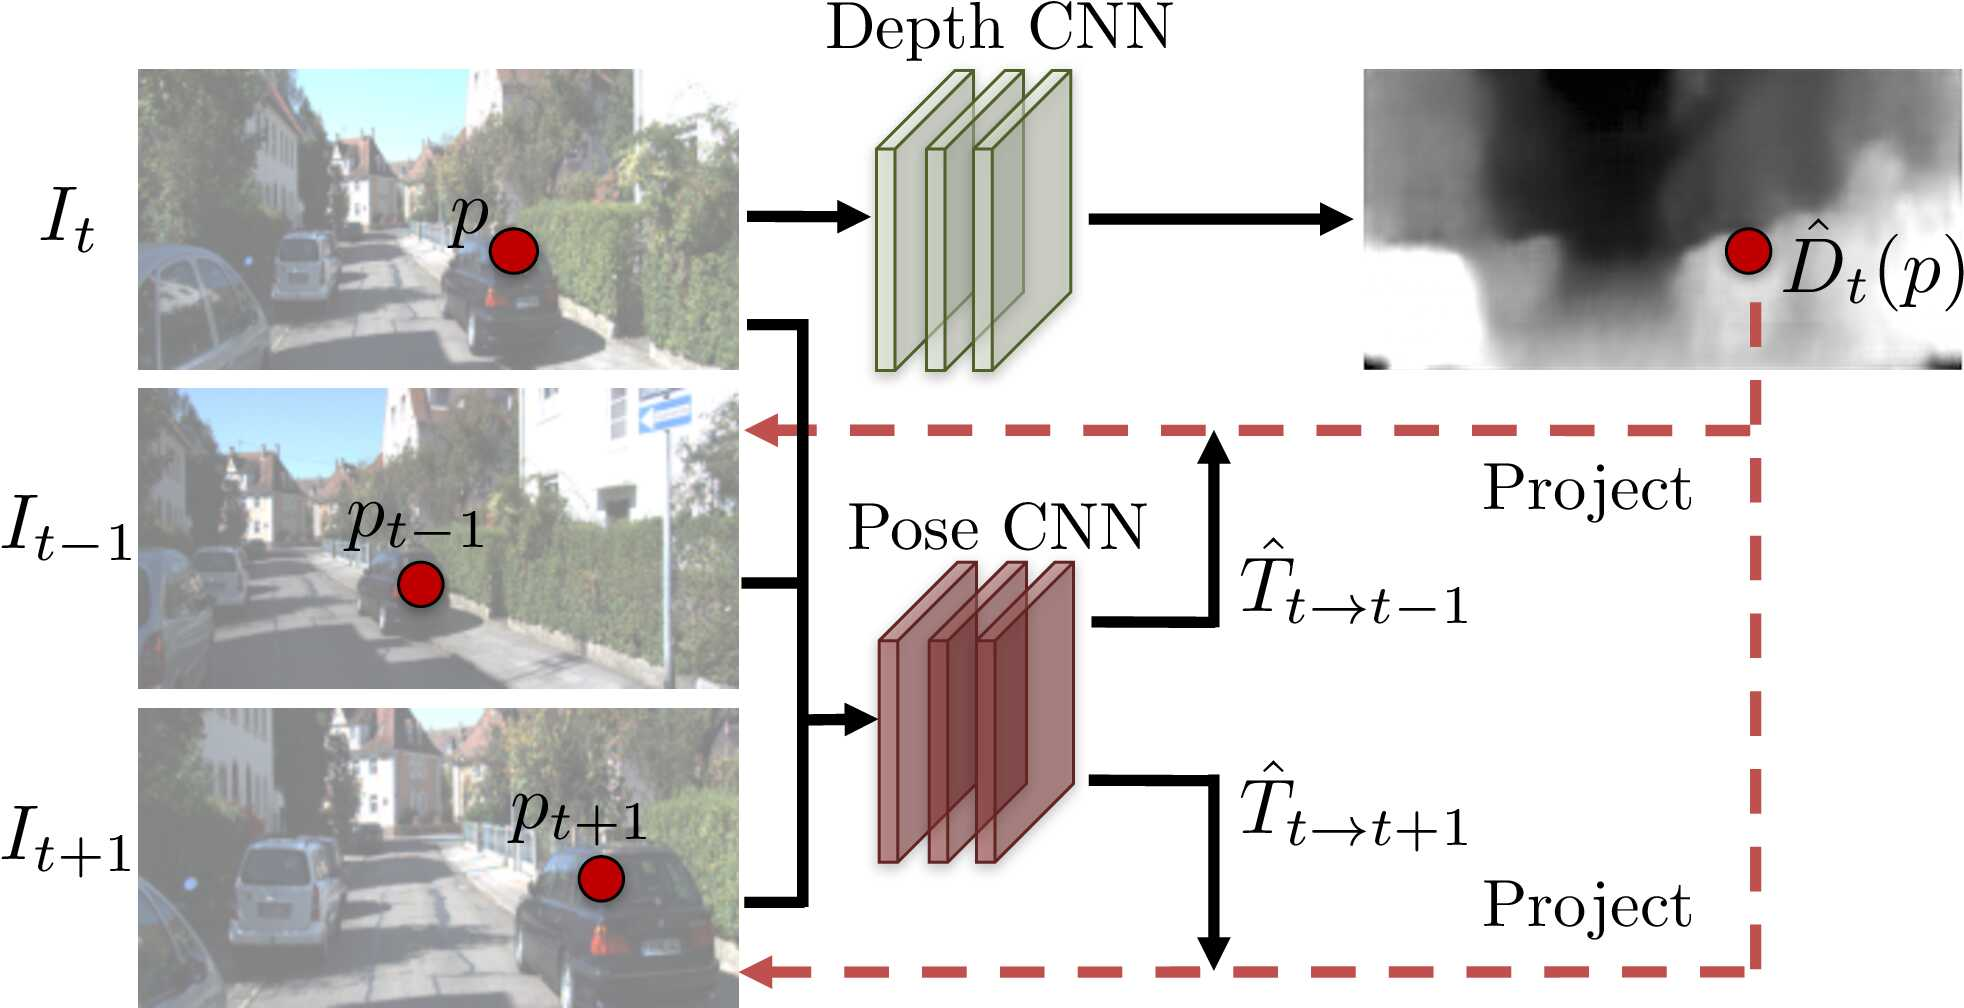
\includegraphics[width=0.5\linewidth]{./img/_sfmlearner.jpg}
            \caption{SfMLearner with two nearby images}
        \end{figure}
\end{description}


\subsection{Depth Pro}

\begin{description}
    \item[Depth Pro] \marginnote{Depth Pro}
        Extension of SfMLearner trained using more datasets.
\end{description}